\section{Simulation Analysis}
\label{sec:simulation}
\paragraph{}
\par For this simulation analysis, it is convenient to represent graphically, with  \textit{LTSpice}, the studied circuit, that can be seen in the following figure.

\begin{figure}[H]
    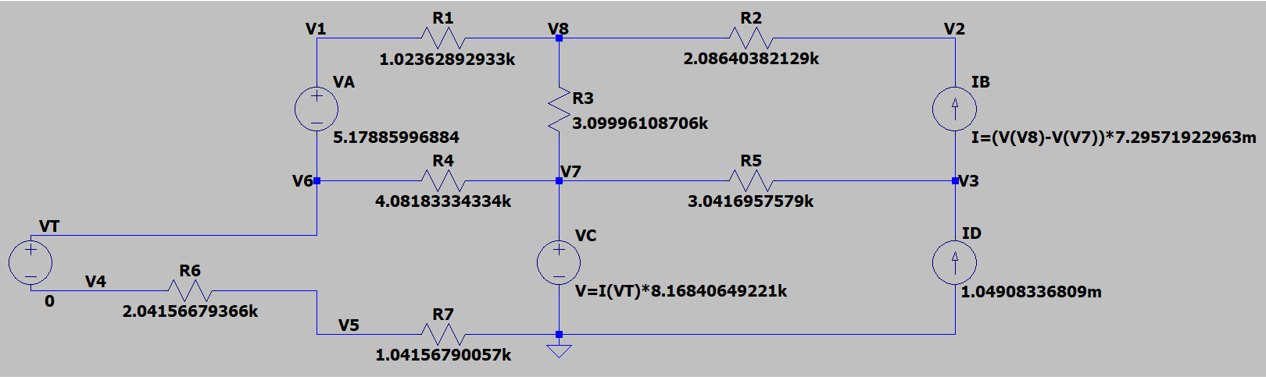
\includegraphics[width=0.8\linewidth]{CircuitLTSpice.png}
    \centering
    \caption{Circuit represented through \textit{LTSpice}}
    \label{circuitsim}
\end{figure}

\par $V_T$ is set to 0 meaning it will function as an ammeter. This is strictly for the purpose of the simulation. In the \textit{Spice} language, in particular in the \textit{NGSpice} software, for a current-controled voltage source there is an input that requires the current, which is controling the voltage source. We can measure that current by inserting an independent voltage source set to 0, making it possible to determine the current that is flowing in that branch without disturbing the system.
The $V_T$ source will be connected to 2 nodes that have the same voltage ($V_6$ and $V_4$), so, although both nodes are used in the simulation, for theoretical analysis one of them was supressed. For coherence purposes it was decided that the same numeration would be used in all models, so we decided to supress $V_4$, therefore not showing it in any analysis.


\par Running the simulation with \textit{NGSpice} we obtained the following results shown in Table~\ref{tab:op}. 

\begin{table}[H]
  \centering
  \begin{tabular}{|l|r|}
    \hline    
    {\bf Name} & {\bf Value [A or V]} \\ \hline
    \input{../sim/op_tab}
  \end{tabular}
  \caption{Operating point. A variable preceded by @ is of type {\em current}
    and expressed in Ampere; other variables are of type {\it voltage} and expressed in
    Volt.}
  \label{tab:op}
\end{table}

\par The data provided by the simulation is enough to solve all the circuit.
That being said, some values need some work so they can be compared. For instance, $V_7$ can be associated  to $V_c$, because $V_c$ imposes the voltage between the ground and $V_7$ implying that $V_7$ equals to $V_c$. $V_a$ is known data, therefore no calculations are executed. Also:

\begin{equation}
	V_b=V_{8}-V_{7}
\end{equation}

\par For the calculations of the currents we can assume that $I_{R_{1}}$ and $I_{R_{6}}$ are equal to $I_a$ and $I_c$, respectively. The current $I_b$ is the current in "g1", the voltage-controlled current source. Once again $I_d$ is a known data.
\par Due to linearity of the resistors, all voltages and currents can be determined knowing the resistance of the resistors, which is given.
\par Finally we can say the circuit has been solved and the results are the following:
\begin{table}[H]
    \centering
    \begin{tabular}{|c|c|}
    \hline
        $I_a$ & 2.40136e-04\\ \hline
        $I_b$ & 2.51245e-04\\ \hline
        $I_c$ & 9.76838e-04\\ \hline
        $V_b$ & 3.4437e-02\\ \hline
        $V_c$ & 7.979210e+00\\ \hline
    \end{tabular}
    \caption{Table of results for the simulation in A and V}
\end{table}







